
\documentclass[a4paper,12pt]{article}
%%%%%%%%%%%%%%%%%%%%%%%%%%%%%%%%%%%%%%%%%%%%%%%%%%%%%%%%%%%%%%%%%%%%%%%%%%%%%%%%%%%%%%%%%%%%%%%%%%%%%%%%%%%%%%%%%%%%%%%%%%%%%%%%%%%%%%%%%%%%%%%%%%%%%%%%%%%%%%%%%%%%%%%%%%%%%%%%%%%%%%%%%%%%%%%%%%%%%%%%%%%%%%%%%%%%%%%%%%%%%%%%%%%%%%%%%%%%%%%%%%%%%%%%%%%%
\usepackage{eurosym}
\usepackage{vmargin}
\usepackage{amsmath}
\usepackage{graphics}
\usepackage{epsfig}
\usepackage{framed}
\usepackage{subfigure}
\usepackage{fancyhdr}

\setcounter{MaxMatrixCols}{10}
%TCIDATA{OutputFilter=LATEX.DLL}
%TCIDATA{Version=5.00.0.2570}
%TCIDATA{<META NAME="SaveForMode"CONTENT="1">}
%TCIDATA{LastRevised=Wednesday, February 23, 201113:24:34}
%TCIDATA{<META NAME="GraphicsSave" CONTENT="32">}
%TCIDATA{Language=American English}

\pagestyle{fancy}
\setmarginsrb{20mm}{0mm}{20mm}{25mm}{12mm}{11mm}{0mm}{11mm}
\lhead{MA4128} \rhead{Kevin O'Brien} \chead{Logistic Regression} %\input{tcilatex}


\begin{document}

\section{Odds and Odds Ratio}
\begin{itemize}
	\item Logistic regression calculates changes in the log odds of the dependent,
	not changes in the dependent value as OLS regression does. For a dichotomous variable the
	odds of membership of the target group are equal to the probability of membership in the
	target group divided by the probability of membership in the other group.
\item Odds value can
	range from 0 to infinity and tell you how much more likely it is that an observation is a
	member of the target group rather than a member of the other group. If the probability is
	0.80, the odds are 4 to 1 or 0.80/0.20; if the probability is 0.25, the odds are .33 (0.25/0.75).
	
\item If the probability of membership in the target group is 0.50, the odds are 1 to 1 (0.50/0.50), as
	in coin tossing when both outcomes are equally likely.
	
\item Another important concept is the odds ratio (OR), which estimates the change in the
	odds of membership in the target group for a one unit increase in the predictor. It is calculated by using the regression coefficient of the predictor as the exponent. Suppose we were predicting exam success by a maths competency
	predictor with an estimate b = 2.69. Thus the odds ratio is exp(2.69) or 14.73. Therefore the odds of passing
	are 14.73 times greater for a student, for example, who had a pre-test score of 5, than for a
	student whose pre-test score was 4.
\end{itemize}

%--------------------------------------------------------%

	%------------------------------------------------------------------------------------------------------------------------- %
\subsection{Odds}
\begin{itemize}
	\item 	The odds in favor of an event or a proposition are the ratio of the probability that an event will happen to the probability that it will not happen.
	\item 		'Odds' are an expression of relative probabilities. Often 'odds' are quoted as odds against, rather than as odds in favor of, because of the possibility of confusion of the latter with the fractional probability of an event occurring.
	\[ \operatorname{Odds} = \frac{p}{1-p} \]
	
	
	
	
	
	
	
	
	\item 	Loglinear models essentially define a pattern of odds ratios, apply the marginals to them, and compare the resulting table with the observed table, in pretty much the same way we apply the Pearson  $\chi^2$ test for association. The big difference is the pattern we define can be much more complicated than independence.
\end{itemize}


\[ \hat{Y} = \frac{\mbox{Odds}}{1+\mbox{Odds}} \]
%---------------------------------------------------------- %

\subsection{Odds and Odds Ratio}
Logistic regression calculates changes in the log odds of the dependent,
not changes in the dependent value as OLS regression does. For a dichotomous variable the
odds of membership of the target group are equal to the probability of membership in the
target group divided by the probability of membership in the other group. Odds value can
range from 0 to infinity and tell you how much more likely it is that an observation is a
member of the target group rather than a member of the other group. If the probability is
0.80, the odds are 4 to 1 or 0.80/0.20; if the probability is 0.25, the odds are .33 (0.25/0.75).

If the probability of membership in the target group is 0.50, the odds are 1 to 1 (0.50/0.50), as
in coin tossing when both outcomes are equally likely.

Another important concept is the odds ratio (OR), which estimates the change in the
odds of membership in the target group for a one unit increase in the predictor. It is calculated by using the regression coefficient of the predictor as the exponent. Suppose we were predicting exam success by a maths competency
predictor with an estimate b = 2.69. Thus the odds ratio is exp(2.69) or 14.73. Therefore the odds of passing
are 14.73 times greater for a student, for example, who had a pre-test score of 5, than for a
student whose pre-test score was 4.
%--------------------------------------------------------%


\subsection{Confidence Intervals for Odds Ratios}
\begin{itemize}
	\item Many statistical implementations of logistic regression include Confidence Intervals for the odds ratios.
	Odds ratios whose confidence limits exclude 1 are statistically significant.
	\item The odds ratio is referred to in SPSS as \texttt{\textbf{Exp(B)}}, the exponentiation of the B coefficient
\end{itemize}



\subsection{The Logistic Regression Equation}
The form of the logistic regression equation is:
\begin{framed}
	\[ \mbox{logit}[p(x)] =  log \left(\frac{p(x)}{1-p(x)} \right) = b_0 + b_1x_1 + b_2x_2 + b_3x_3 + \ldots \]
\end{framed}
This looks just like a linear regression and although logistic regression finds a �best
fitting� equation, just as linear regression does, the principles on which it does so are
rather different. Instead of using a least-squared deviations criterion for the best fit, it
uses a maximum likelihood method, which maximizes the probability of getting the
observed results given the fitted regression coefficients. A consequence of this is that the
goodness of fit and overall significance statistics used in logistic regression are different
from those used in linear regression.

The probability that a case is in a particular category,p, can be calculated with the following formula (which is simply another rearrangement of the previous formula).

\[p = \frac{exp(b_0 + b_1x_1 + b_2x_2 + b_3x_3 + \ldots)}{1 + exp(b_0 + b_1x_1 + b_2x_2 + b_3x_3 + \ldots)}\]

\newpage


\section{Review of Logistic Regression}
% http://www.nesug.org/proceedings/nesug06/an/da26.pdf
% http://www.ccsr.ac.uk/publications/teaching/blr.pdf
% http://www.southampton.ac.uk/ghp3/docs/unicef/presentation7.1a.pdf
% ftp://public.dhe.ibm.com/software/analytics/spss/documentation/statistics/20.0/en/client/Manuals/IBM_SPSS_Regression.pdf
% http://www.umass.edu/statdata/statdata/data/

\subsection*{Logistic Regression: Logit Transformation}
%http://data.princeton.edu/wws509/notes/c3.pdf

The logit transformation is given by the following formula: 
\[ \eta_i = \mbox{logit}(\pi_i)  = \mbox{log}\left( \frac{\pi_i}{1- \pi_i} \right) \]

\noindent 
The inverse of the logit transformation is given by the following formula: 
\[ \pi_i = \mbox{logit}^{-1}(\eta_i)  =  \frac{e^{\eta_i}}{1 + e^{\eta_i}} \]

%---------------------------%




\subsection*{Logistic function} 

The logistic function, with $\beta_0 + \beta_1 x$ on the horizontal axis and $\pi(x)$ on the vertical axis
An explanation of logistic regression begins with an explanation of the logistic function, which always takes on values between zero and one:
\[
F(t) = \frac{e^t}{e^t+1} = \frac{1}{1+e^{-t}},
\]
and viewing $t$ as a linear function of an explanatory variable x (or of a linear combination of explanatory variables), the logistic function can be written as:
\[\pi(x) = \frac{e^{(\beta_0 + \beta_1 x)}} {e^{(\beta_0 + \beta_1 x)} + 1} = \frac {1} {1+e^{-(\beta_0 + \beta_1 x)}}.
\]
This will be interpreted as the probability of the dependent variable equalling a ``success" or ``case" rather than a failure or non-case. We also define the inverse of the logistic function, the logit:
\[g(x) = \log \frac {\pi(x)} {1 - \pi(x)} = \beta_0 + \beta_1 x ,
\]and equivalently:
\[\frac{\pi(x)} {1 - \pi(x)} = e^{(\beta_0 + \beta_1 x)}.
\]
%======================================================%


%---------------------------%



\subsection{About logits}


There is a direct relationship between the coefficients produced by \textbf{logit} and the odds ratios produced by the logistic procedure.  First, let's define what is meant by a logit:  A logit is defined as the log base e (log) of the odds,
\[logit(p) = log(odds) = log(p/q)\]
Logistic regression is in reality ordinary regression using the logit as the response variable,

\[logit(p) = log(p/q) = b_0 + b_1X\]

This means that the coefficients in logistic regression are in terms of the log odds, that is, the coefficient 1.694596 implies that a one unit change in gender results in a 1.694596 unit change in the log of the odds.  

Equation [3] can be expressed in odds by getting rid of the log.  This is done by taking e to the power for both sides of the equation.
\[ p/q = e^{b_0 + b_1}\]
The end result of all the mathematical manipulations is that the odds ratio can be computed by raising e to the power of the logistic coefficient,
\[OR = e^b = e^1.694596 = 5.44\]


%---------------------------------------------------------- %
\newpage


\subsection{The Sigmoid Graph}
\begin{itemize}
	\item While logistic regression gives each predictor (IV) a coefficient \textbf{b} which measures its
	independent contribution to variations in the dependent variable, the dependent variable
	can only take on one of the two values: 0 or 1.
	
	\item	What we want to predict from a knowledge of relevant independent variables and coefficients is therefore not a numerical value of a
	dependent variable as in linear regression, but rather the probability (p) that it is 1 rather
	than 0 (belonging to one group rather than the other). 
	\item But even to use probability as the dependent variable is unsound, mainly because numerical predictors may be unlimited in range.
	\item  If we expressed p as a linear function of investment, we might then find ourselves predicting that p is greater than 1 (which cannot be true, as
	probabilities can only take values between 0 and 1). 
	
	\item Additionally, because logistic regression
	has only two y values � in the category or not in the category � a straight line best fit (as in
	linear regression) is not possible to draw.
\end{itemize}

\subsection{The Sigmoid Graph}
While logistic regression gives each predictor (IV) a coefficient \textbf{b} which measures its
independent contribution to variations in the dependent variable, the dependent variable
can only take on one of the two values: 0 or 1.

What we want to predict from a knowledge of relevant independent variables and coefficients is therefore not a numerical value of a
dependent variable as in linear regression, but rather the probability (p) that it is 1 rather
than 0 (belonging to one group rather than the other). But even to use probability as the dependent variable is unsound, mainly because numerical predictors may be unlimited in range. If we expressed p as a linear function of investment, we might then find ourselves predicting that p is greater than 1 (which cannot be true, as
probabilities can only take values between 0 and 1). Additionally, because logistic regression
has only two y values � in the category or not in the category � a straight line best fit (as in
linear regression) is not possible to draw.
\subsubsection{Hypothetical Example}
Consider the following hypothetical example:
200 accountancy first year students are graded on a pass-fail dichotomy on the end of the
semester accountancy exam. At the start of the course, they all took a maths pre-test with
results reported in interval data ranging from 0�50 � the higher the pretest score the more
competency in maths. Logistic regression is applied to determine the relationship between
maths pretest score (IV or predictor) and whether a student passed the course (DV). Students
who passed the accountancy course are coded 1 while those who failed are coded 0.
\begin{center}
	\begin{figure}
		% Requires \usepackage{graphicx}
		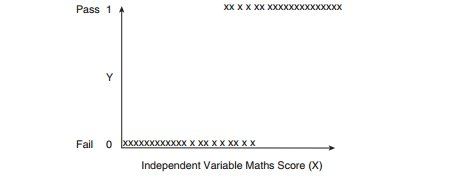
\includegraphics[scale=0.8]{images/Logistic1}\\
		\caption{Accountancy Exam Results}
	\end{figure}
\end{center}

We can see from Figure 1 of the plotted �x�s� that there is somewhat greater likelihood
that those who obtained above average to high score on the maths test passed the accountancy course, while below average to low scorers tended to fail. There is also an overlap in
the middle area. But if we tried to draw a straight (best fitting) line, as with linear regression,
it just would not work, as intersections of the maths results and pass/fail accountancy results
form two lines of x�s, as in Figure 1.
%
%\begin{figure}
%  % Requires \usepackage{graphicx}
%  \includegraphics[width=0.40]{Logistic2.jpeg}\\
%  \caption{Figure 2}
%\end{figure}
\begin{center}
	\begin{figure}
		% Requires \usepackage{graphicx}
		\includegraphics[scale=0.8]{images/Logistic2}\\
		\caption{Accountancy Exam Results - Fitted Curve}
	\end{figure}
\end{center}

The solution is to convert or transform these results into probabilities. We might compute
the average of the Y values at each point on the X axis. We could then plot the probabilities
of Y at each value of X and it would look something like the wavy graph line superimposed
on the original data in Figure 2. This is a smoother curve, and it is easy to see that the
probability of passing the accountancy course (Y axis) increases as values of X increase.
What we have just done is transform the scores so that the curve now fits a cumulative
probability curve, i.e. adding each new probability to the existing total. As you can see, this
curve is not a straight line; it is more of an s-shaped curve (A sigmoid curve).

Predicted values are interpreted as probabilities and are now not just two conditions with a value of either 0 or 1 but continuous data that can take any value from 0 to 1.
The slope of the curve in Figure 2 is low at the lower and upper extremes of the
independent variable and greatest in the middle where it is most sensitive. In the middle, of
course, are a number of cases that are out of order, in the sense that there is an overlap with
average maths scores in both accountancy pass and fail categories, while at the extremes are
cases which are almost universally allocated to their correct group. The outcome is not a prediction of a Y value, as in linear regression, but a probability of belonging to one of two conditions
of Y, which can take on any value between 0 and 1 rather than just 0 and 1 in Figure 1.


\subsubsection{Log transformation}
Unfortunately a further mathematical transformation � a log transformation � is needed
to normalize the distribution. Transformations, such as log transformations and
square root transformations transform non-normal/skewed distributions closer to normality.

This log transformation of the p values to a log distribution enables us to create a link with the normal regression equation. The log distribution (or logistic transformation of p) is also called the logit of p or \textbf{\textit{logit(p)}}.


%-------------------------------------------%


\subsection{Hypothetical Example}
\begin{itemize}
	\item 	Consider the following hypothetical example:
	200 accountancy first year students are graded on a pass-fail dichotomy on the end of the
	semester accountancy exam. 
	\item At the start of the course, they all took a maths pre-test with
	results reported in interval data ranging from 0�50 � the higher the pretest score the more
	competency in maths. 
	\item Logistic regression is applied to determine the relationship between
	maths pretest score (IV or predictor) and whether a student passed the course (DV). 
	\item Students
	who passed the accountancy course are coded 1 while those who failed are coded 0.
\end{itemize}

\begin{center}
	\begin{figure}[h!]
		% Requires \usepackage{graphicx}
		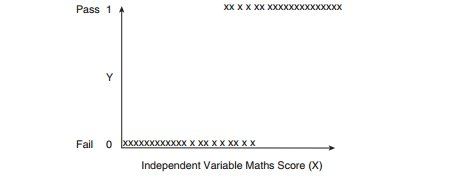
\includegraphics[scale=1.1]{images/Logistic1}\\
		\caption{Accountancy Exam Results}
	\end{figure}
\end{center}

We can see from Figure 1 of the plotted �x�s� that there is somewhat greater likelihood
that those who obtained above average to high score on the maths test passed the accountancy course, while below average to low scorers tended to fail. There is also an overlap in
the middle area. But if we tried to draw a straight (best fitting) line, as with linear regression,
it just would not work, as intersections of the maths results and pass/fail accountancy results
form two lines of x�s, as in Figure 1.
%
%\begin{figure}
%  % Requires \usepackage{graphicx}
%  \includegraphics[width=0.40]{Logistic2.jpeg}\\
%  \caption{Figure 2}
%\end{figure}
\begin{center}
	\begin{figure}
		% Requires \usepackage{graphicx}
		\includegraphics[scale=0.8]{images/Logistic2}\\
		\caption{Accountancy Exam Results - Fitted Curve}
	\end{figure}
\end{center}
\begin{itemize}
	\item 	The solution is to convert or transform these results into probabilities. We might compute
	the average of the Y values at each point on the X axis. We could then plot the probabilities
	of Y at each value of X and it would look something like the wavy graph line superimposed
	on the original data in Figure 2. This is a smoother curve, and it is easy to see that the
	probability of passing the accountancy course (Y axis) increases as values of X increase.
	\item What we have just done is transform the scores so that the curve now fits a cumulative
	probability curve, i.e. adding each new probability to the existing total. As you can see, this
	curve is not a straight line; it is more of an s-shaped curve (A sigmoid curve).
	
	\item Predicted values are interpreted as probabilities and are now not just two conditions with a value of either 0 or 1 but continuous data that can take any value from 0 to 1.
	The slope of the curve in Figure 2 is low at the lower and upper extremes of the
	independent variable and greatest in the middle where it is most sensitive. 
	\item In the middle, of
	course, are a number of cases that are out of order, in the sense that there is an overlap with
	average maths scores in both accountancy pass and fail categories, while at the extremes are
	cases which are almost universally allocated to their correct group. The outcome is not a prediction of a Y value, as in linear regression, but a probability of belonging to one of two conditions
	of Y, which can take on any value between 0 and 1 rather than just 0 and 1 in Figure 1.
	
\end{itemize}

%	\subsubsection{Log transformation}
%	Unfortunately a further mathematical transformation � a log transformation � is needed
%	to normalize the distribution. Transformations, such as log transformations and
%	square root transformations transform non-normal/skewed distributions closer to normality.
%	
%	This log transformation of the p values to a log distribution enables us to create a link with the normal regression equation. The log distribution (or logistic transformation of p) is also called the logit of p or \textbf{\textit{logit(p)}}.
%	


\newpage



\subsection{The Logit}
The convention for binomial logistic regression is to code the
dependent class of greatest interest as 1 and the other class as 0, because the coding will
affect the odds ratios and slope estimates.

The logit(p) is the log (to base e) of the odds ratio or likelihood ratio that the dependent
variable is 1. In symbols it is defined as:
\[ logit(p) = ln \left(\frac{p}{(1-p)}\right) \]

Whereas p can only range from 0 to 1, logit(p) scale ranges from negative infinity to positive
infinity and is symmetrical around the logit of 0.5 (which is zero)


\subsection{Odds}
The odds in favor of an event or a proposition are the ratio of the probability that an event will happen to the probability that it will not happen.
'Odds' are an expression of relative probabilities. Often 'odds' are quoted as odds against, rather than as odds in favor of, because of the possibility of confusion of the latter with the fractional probability of an event occurring.
\[ \operatorname{Odds} = \frac{p}{1-p} \]

\subsubsection{Example}
There are 5 pink marbles, 2 blue marbles, and 8 purple marbles.

\begin{itemize}
	\item What is the probability of picking a blue marble? (Answer: 2/15).
	\item What are the odds in favor of picking a blue marble? (Answer: 2/13).
\end{itemize}



%-------------------------------------------%
\subsection{Log-Odds}
As an alternative to modeling the value of the outcome, logistic regression focuses instead upon the
relative probability (odds) of obtaining a given result category. The natural logarithm of the odds is
linear across most of its range, allowing us to continue using many of the methods developed for linear models.
The result of this type of regression can be expressed as follows:
\[ \operatorname{Ln} \left[ \frac{p}{1-p} \right] = b_0 + b_1x_1 + b_2x_2 + b_3x_3 \ldots b_kx_k + e \]

%-------------------------------------------%


\subsection*{Logits}
In logistic regression, the logit may be computed in a manner similar to linear regression:
\[ \eta_i = \beta_0 + \beta_1x_1 + \beta_2x_2 + \ldots  \]

%---------------------------%




\subsection{Logistic function}

The logistic function of any number is given by the inverse-logit:

\[\operatorname{logit}^{-1}(\alpha) = \frac{1}{1 + \operatorname{exp}(-\alpha)} = \frac{\operatorname{exp}(\alpha)}{1 + \operatorname{exp}(\alpha)}\]

%-------------------------------------------%
%--------------------------------------------%
\subsection{Log-Odds}
As an alternative to modeling the value of the outcome, logistic regression focuses instead upon the
relative probability (odds) of obtaining a given result category. The natural logarithm of the odds is
linear across most of its range, allowing us to continue using many of the methods developed for linear models.
The result of this type of regression can be expressed as follows:
\[ \operatorname{Ln} \left[ \frac{p}{1-p} \right] = b_0 + b_1x_1 + b_2x_2 + b_3x_3 \ldots b_kx_k + e \]


\subsection{Introduction to the Odds Ratio}
Let's begin with probability. Suppose that the probability of success is 0.8, thus
p = 0.8
Then the probability of failure is
\[q = 1 - p = 0.2\]
The odds of success are defined as
\[odds(success) = p/q = 0.8/0.2 = 4\]
that is, the odds of success are 4 to 1. The odds of failure would be
\[odds(failure) = q/p = .2/.8 = .25\]
This looks a little strange but it is really saying that the odds of failure are 1 to 4.  The odds of success and the odds of failure are just reciprocals of one another, i.e., 1/4 = 0.25 and 1/0.25 = 4. 
	

\subsection{About logits}


There is a direct relationship between the coefficients produced by \textbf{logit} and the odds ratios produced by the logistic procedure.  First, let's define what is meant by a logit:  A logit is defined as the log base e (log) of the odds,
\[logit(p) = log(odds) = log(p/q)\]
Logistic regression is in reality ordinary regression using the logit as the response variable,

\[logit(p) = log(p/q) = b_0 + b_1X\]

This means that the coefficients in logistic regression are in terms of the log odds, that is, the coefficient 1.694596 implies that a one unit change in gender results in a 1.694596 unit change in the log of the odds.  

Equation [3] can be expressed in odds by getting rid of the log.  This is done by taking e to the power for both sides of the equation.
\[ p/q = e^{b_0 + b_1}\]
The end result of all the mathematical manipulations is that the odds ratio can be computed by raising e to the power of the logistic coefficient,
\[OR = e^b = e^1.694596 = 5.44\]


%---------------------------------------------------------- %
\newpage


\subsection{The Sigmoid Graph}
While logistic regression gives each predictor (IV) a coefficient \textbf{b} which measures its
independent contribution to variations in the dependent variable, the dependent variable
can only take on one of the two values: 0 or 1.

What we want to predict from a knowledge of relevant independent variables and coefficients is therefore not a numerical value of a
dependent variable as in linear regression, but rather the probability (p) that it is 1 rather
than 0 (belonging to one group rather than the other). But even to use probability as the dependent variable is unsound, mainly because numerical predictors may be unlimited in range. If we expressed p as a linear function of investment, we might then find ourselves predicting that p is greater than 1 (which cannot be true, as
probabilities can only take values between 0 and 1). Additionally, because logistic regression
has only two y values � in the category or not in the category � a straight line best fit (as in
linear regression) is not possible to draw.
\subsection{Hypothetical Example}
\begin{itemize}
	\item 	Consider the following hypothetical example:
	200 accountancy first year students are graded on a pass-fail dichotomy on the end of the
	semester accountancy exam. 
	\item At the start of the course, they all took a maths pre-test with
	results reported in interval data ranging from 0�50 � the higher the pretest score the more
	competency in maths. 
	\item Logistic regression is applied to determine the relationship between
	maths pretest score (IV or predictor) and whether a student passed the course (DV). 
	\item Students
	who passed the accountancy course are coded 1 while those who failed are coded 0.
\end{itemize}

\begin{center}
	\begin{figure}[h!]
		% Requires \usepackage{graphicx}
		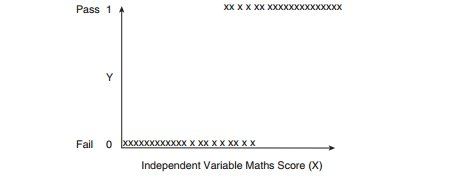
\includegraphics[scale=1.1]{images/Logistic1}\\
		\caption{Accountancy Exam Results}
	\end{figure}
\end{center}

We can see from Figure 1 of the plotted �x�s� that there is somewhat greater likelihood
that those who obtained above average to high score on the maths test passed the accountancy course, while below average to low scorers tended to fail. There is also an overlap in
the middle area. But if we tried to draw a straight (best fitting) line, as with linear regression,
it just would not work, as intersections of the maths results and pass/fail accountancy results
form two lines of x�s, as in Figure 1.
%
%\begin{figure}
%  % Requires \usepackage{graphicx}
%  \includegraphics[width=0.40]{Logistic2.jpeg}\\
%  \caption{Figure 2}
%\end{figure}
\begin{center}
	\begin{figure}
		% Requires \usepackage{graphicx}
		\includegraphics[scale=0.8]{images/Logistic2}\\
		\caption{Accountancy Exam Results - Fitted Curve}
	\end{figure}
\end{center}
\begin{itemize}
	\item 	The solution is to convert or transform these results into probabilities. We might compute
	the average of the Y values at each point on the X axis. We could then plot the probabilities
	of Y at each value of X and it would look something like the wavy graph line superimposed
	on the original data in Figure 2. This is a smoother curve, and it is easy to see that the
	probability of passing the accountancy course (Y axis) increases as values of X increase.
	\item What we have just done is transform the scores so that the curve now fits a cumulative
	probability curve, i.e. adding each new probability to the existing total. As you can see, this
	curve is not a straight line; it is more of an s-shaped curve (A sigmoid curve).
	
	\item Predicted values are interpreted as probabilities and are now not just two conditions with a value of either 0 or 1 but continuous data that can take any value from 0 to 1.
	The slope of the curve in Figure 2 is low at the lower and upper extremes of the
	independent variable and greatest in the middle where it is most sensitive. 
	\item In the middle, of
	course, are a number of cases that are out of order, in the sense that there is an overlap with
	average maths scores in both accountancy pass and fail categories, while at the extremes are
	cases which are almost universally allocated to their correct group. The outcome is not a prediction of a Y value, as in linear regression, but a probability of belonging to one of two conditions
	of Y, which can take on any value between 0 and 1 rather than just 0 and 1 in Figure 1.
	
\end{itemize}

%	\subsubsection{Log transformation}
%	Unfortunately a further mathematical transformation � a log transformation � is needed
%	to normalize the distribution. Transformations, such as log transformations and
%	square root transformations transform non-normal/skewed distributions closer to normality.
%	
%	This log transformation of the p values to a log distribution enables us to create a link with the normal regression equation. The log distribution (or logistic transformation of p) is also called the logit of p or \textbf{\textit{logit(p)}}.
%	


\newpage
\subsection*{South Africa Heart Disease Data Example}

\begin{framed}
	A retrospective sample of males in a heart-disease high-risk region
	of the Western Cape, South Africa. There are roughly two controls per
	case of CHD. Many of the CHD positive men have undergone blood
	pressure reduction treatment and other programs to reduce their risk
	factors after their CHD event. In some cases the measurements were
	made after these treatments. These data are taken from a larger
	dataset, described in  Rousseauw et al, 1983, South African Medical
	Journal. 
	
\end{framed}
%Load the South Africa Heart Disease Data and create training and test sets with
%the following code:
%\begin{framed}
%	\begin{verbatim}
%	install.packages("ElemStatLearn")
%	library(ElemStatLearn)
%	data(SAheart)
%	
%	set.seed(8484)
%	train = sample(1:dim(SAheart)[1],
%	size=dim(SAheart)[1]/2,replace=F)
%	trainSA = SAheart[train,]
%	testSA = SAheart[-train,]
%	
%	\end{verbatim}
%\end{framed}

\noindent \textbf{Exercise}\\Fit a logistic regression model with
\begin{itemize}
	\item \textit{Coronary Heart Disease} (\texttt{chd}) as the
	dependent variable
	
	\item \textit{age at onset, current alcohol consumption, obesity levels,
		cumulative tabacco, type-A behavior}, and \textit{low density lipoprotein cholesterol} as predictor variables. 
\end{itemize} 
{
	\large
	
	\begin{verbatim}
	> head(SAheart)
	sbp tobacco  ldl adiposity famhist typea obesity alcohol age chd
	1 160   12.00 5.73     23.11 Present    49   25.30   97.20  52   1
	2 144    0.01 4.41     28.61  Absent    55   28.87    2.06  63   1
	3 118    0.08 3.48     32.28 Present    52   29.14    3.81  46   0
	4 170    7.50 6.41     38.03 Present    51   31.99   24.26  58   1
	5 134   13.60 3.50     27.78 Present    60   25.99   57.34  49   1
	6 132    6.20 6.47     36.21 Present    62   30.77   14.14  45   0
	...
	...
	\end{verbatim}
	
}
\noindent Calculate the misclassification rate for your model using this model
% function and a prediction on the "response" scale:

%\noindent What is the misclassification rate on the training set? What is the
%misclassification rate on the test set?
%\begin{framed}
%	\begin{verbatim}
%	head(SAheart)
%	
%	lr1 <- glm(chd ~ age + alcohol + obesity + 
%	tobacco + typea + ldl, data=trainSA, 
%	family="binomial")
%	
%	lr1.train.predict <- predict(lr1, type="response")
%	
%	missclass.lr1.train <- missClass(trainSA$chd, 
%	lr1.train.predict)
%	
%	lr1.test.predict <- predict(lr1, newdata=testSA, 
%	type="response")
%	
%	missclass.lr1.test <- missClass(testSA$chd, 
%	lr1.test.predict)
%	\end{verbatim}
%\end{framed}


\newpage
%-------------------------------------------------------%


\section{Introduction to the Odds Ratio}
Let's begin with probability.  Let's say that the probability of success is 0.8, thus
p = 0.8
Then the probability of failure is
\[q = 1 - p = 0.2\]
The odds of success are defined as
\[odds(success) = p/q = 0.8/0.2 = 4\]
that is, the odds of success are 4 to 1. The odds of failure would be
\[odds(failure) = q/p = .2/.8 = .25\]
This looks a little strange but it is really saying that the odds of failure are 1 to 4.  The odds of success and the odds of failure are just reciprocals of one another, i.e., 1/4 = .25 and 1/.25 = 4. 


Next, we will add another variable to the equation so that we can compute an odds ratio.

\textbf{Another example}

Suppose that seven out of 10 males are admitted to an engineering school while three of 10 females are admitted. 

\begin{itemize}
	\item The probabilities for admitting a male are,
	p = 7/10 = .7      ( q = 1 - .7 = .3)
	\item Here are the same probabilities for females,
	p = 3/10 = .3       (q = 1 - .3 = .7)
\end{itemize}
Now we can use the probabilities to compute the admission odds for both males and females,
\begin{itemize}
	\item odds(male) = .7/.3 = 2.33333
	\item odds(female) = .3/.7 = .42857
\end{itemize}
Next, we compute the odds ratio for admission,
\[OR = 2.3333/0.42857 = 5.44\]
Thus, for a male, the odds of being admitted are 5.44 times as large than the odds for a female being admitted.

\subsection{About logits}


There is a direct relationship between the coefficients produced by \textbf{logit} and the odds ratios produced by the logistic procedure.  First, let's define what is meant by a logit:  A logit is defined as the log base e (log) of the odds,
\[logit(p) = log(odds) = log(p/q)\]
Logistic regression is in reality ordinary regression using the logit as the response variable,

\[logit(p) = a + bX\]
\[log(p/q) = a + bX\]
This means that the coefficients in logistic regression are in terms of the log odds, that is, the coefficient 1.694596 implies that a one unit change in gender results in a 1.694596 unit change in the log of the odds.  

Equation [3] can be expressed in odds by getting rid of the log.  This is done by taking e to the power for both sides of the equation.
\[ p/q = e^{a + bX}\]
The end result of all the mathematical manipulations is that the odds ratio can be computed by raising e to the power of the logistic coefficient,
\[OR = e^b = e^1.694596 = 5.44\]
%------------------------------------------------------------------------------------------------------------------------- %
\subsection{Logistic Regression: Odds Ratio}
What are odds?
The odds of outcome 1 versus outcome 2 are the probability (or frequency) of outcome 1 divided by the probability (or frequency) of outcome 2.


\[ \hat{Y} = \frac{\mbox{Odds}}{1+\mbox{Odds}} \]


Loglinear models essentially define a pattern of odds ratios, apply the marginals to them, and compare the resulting table with the observed table, in pretty much the same way we apply the Pearson  $\chi^2$ test for association. The big difference is the pattern we define can be much more complicated than independence.

%---------------------------------------------------------- %
	\section{Logistic Regression}
Logistic regression, also called a logit model, is used to model \textbf{dichotomous outcome} variables. 
In the logit model the \textbf{log odds} of the outcome is modeled as a linear combination of the predictor variables.

In logistic regression theory, the predicted dependent variable is a function of the probability that a particular subject will be in one of the categories (for example, the probability that a patient has the disease, given his or her set of scores on the predictor variables).
%------------------------------------------------------------------------------------------------------------------------- %
\subsection{Odds}
\begin{itemize}
	\item 	The odds in favor of an event or a proposition are the ratio of the probability that an event will happen to the probability that it will not happen.
	\item 		'Odds' are an expression of relative probabilities. Often 'odds' are quoted as odds against, rather than as odds in favor of, because of the possibility of confusion of the latter with the fractional probability of an event occurring.
	\[ \operatorname{Odds} = \frac{p}{1-p} \]
	
	
	
	
	
	
	
	
	\item 	Loglinear models essentially define a pattern of odds ratios, apply the marginals to them, and compare the resulting table with the observed table, in pretty much the same way we apply the Pearson  $\chi^2$ test for association. The big difference is the pattern we define can be much more complicated than independence.
\end{itemize}


\[ \hat{Y} = \frac{\mbox{Odds}}{1+\mbox{Odds}} \]
%---------------------------------------------------------- %


%--------------------------------------------------------%

\subsection{Introduction to the Odds Ratio}
Let's begin with probability. Suppose that the probability of success is 0.8, thus
p = 0.8
Then the probability of failure is
\[q = 1 - p = 0.2\]
The odds of success are defined as
\[odds(success) = p/q = 0.8/0.2 = 4\]
that is, the odds of success are 4 to 1. The odds of failure would be
\[odds(failure) = q/p = .2/.8 = .25\]
This looks a little strange but it is really saying that the odds of failure are 1 to 4.  The odds of success and the odds of failure are just reciprocals of one another, i.e., 1/4 = 0.25 and 1/0.25 = 4. 


\subsection{Confidence Intervals for Odds Ratios}
\begin{itemize}
	\item Many statistical implementations of logistic regression include Confidence Intervals for the odds ratios.
	Odds ratios whose confidence limits exclude 1 are statistically significant.
	\item The odds ratio is referred to in SPSS as \texttt{\textbf{Exp(B)}}, the exponentiation of the B coefficient
\end{itemize}


%-------------------------------------------%


\subsection*{Logits}
In logistic regression, the logit may be computed in a manner similar to linear regression:
\[ \eta_i = \beta_0 + \beta_1x_1 + \beta_2x_2 + \ldots  \]

%---------------------------%




\subsection{Logistic function}

The logistic function of any number is given by the inverse-logit:

\[\operatorname{logit}^{-1}(\alpha) = \frac{1}{1 + \operatorname{exp}(-\alpha)} = \frac{\operatorname{exp}(\alpha)}{1 + \operatorname{exp}(\alpha)}\]

%-------------------------------------------%


%-------------------------------------------%
\subsection{Odds Ratio Example}
These data are taken from the \textbf{\textit{British Election Study 2005}} pre-campaign and
post-election panel data. We will consider the propensity to vote (sometimes called ``turnout") as the
dependent variable, which has 2 categories. 0=did not turn out to vote, 1 turned
out to vote.
% \begin{center}
% \begin{figure}
%  % Requires \usepackage{graphicx}
%  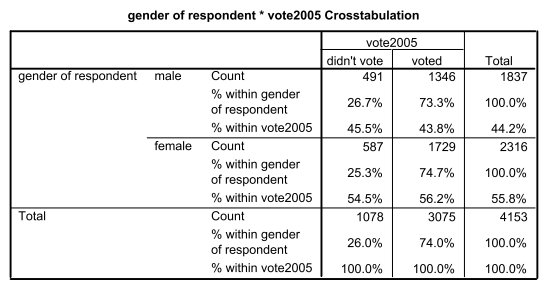
\includegraphics[scale=0.6]{images/LogWeek10A}\\
%  \caption{General Election 2005}
% \end{figure}
% \end{center}

% Image LogWeek10-A
\begin{itemize}
	\item The odds of a male turning out to vote are:
	\[1346/491 = 2.741\]
	\item The odds of female turning out to vote are
	\[1729/587 = 2.945\]
	\item The Odds ratio (female: male) are
	\[(1729/587) / (1346/491) = 1.074\]
	
\end{itemize}

%-------------------------------------------%
\subsection{Logit}
The \textbf{logit} of a number $p$ between 0 and 1 is given by the formula:

\[\operatorname{logit}(p)=\log\left( \frac{p}{1-p} \right) =\log(p)-\log(1-p). \!\]

%-------------------------------------------%



\section{Dummy variables}
When an explanatory variable is categorical we can use \textbf{dummy variables} to contrast
the different categories. For each variable we choose a baseline category and then
contrast all remaining categories with the base line. If an explanatory variable
has k categories, we need k-1 dummy variables to investigate all the differences in
the categories with respect to the dependent variable.

For example suppose the explanatory variable was \textbf{\textit{housing}} coded like this:
\begin{itemize}
	\item[1:] Owner occupier
	\item[2:] renting from a private landlord
	\item[3:] renting from the local authority
\end{itemize}

We would therefore need to choose a baseline category and create two dummy
variables. For example if we chose owner occupier as the baseline category we
would code the dummy variables (House1 and House2) like this

%Tenure: &House1 &House2\\
%Owner occupier &0& 0\\
%Rented private &1 &0\\
%Rented local authority &0 &1\\



%-------------------------------------------%
\subsection{Odds Ratio}
Suppose that in a sample of 100 men, 90 drank wine in the previous week, while in a sample of
100 women only 20 drank wine in the same period. The odds of a man drinking wine are 90 to 10,
or 9:1, while the odds of a
woman drinking wine are only 20 to 80, or 1:4 = 0.25:1. The odds ratio is thus 9/0.25, or 36,
showing that men are much more likely to drink wine than women. The detailed calculation is:
\[{ 0.9/0.1 \over 0.2/0.8}=\frac{\;0.9\times 0.8\;}{\;0.1\times 0.2\;} ={0.72 \over 0.02} = 36.\]
This example also shows how odds ratios are sometimes sensitive in stating relative positions:
in this sample men are 90/20 = 4.5 times more likely to have drunk wine than women, but have 36 times the odds.

The logarithm of the odds ratio, the difference of the logits of the probabilities, tempers this effect, and also makes the measure symmetric with respect to the ordering of groups. For example, using natural logarithms, an odds ratio of 36/1 maps to 3.584, and an odds ratio of 1/36 maps to -3.584.


%%%%%%%%%%%%%%%%%%%%%%%%%%%%%%%%%%%%%%%%%%%%%%%%%%%%%%%%%%%%%%%%%%%%%%%%%%%%%%%%%%%%%%%

%---------------------------%
\subsection{Example 2}
Let us suppose that the probability of survival of a marine species of fauna is dependent on pollution, depth and water temperature. Suppose the logit for the logistic regression was computed as follows:
\[ \eta_i = 0.14 + 0.76x_1 - 0.093x_2 + 1.2x_3  \]
\begin{center}
\begin{tabular}{|c|c|c|}
  \hline
  % after \\: \hline or \cline{col1-col2} \cline{col3-col4} ...
Variables & case 1 & case 2 \\ \hline
Pollution($x_1$) & 6.0 & 1.9 \\
Depth ($x_2$)& 51 & 99 \\
Temp ($x_3$) & 3.0 & 2.9 \\
  \hline
\end{tabular}
\end{center}
Compute the probability of success for both case 1 and case 2.

\begin{itemize}
\item case 1$ \eta_1 = 0.14 + (0.76 \times 6)	- (0.093\times 51) + (1.2\times 3) = 3.557$
\item case 2$ \eta_2 = 0.14 + (0.76 \times 1.9)	- (0.093\times 99) + (1.2\times 2.9) = -4.143$
\end{itemize}

The probabilities for success are therefore:
\[ \pi_1  =  \frac{e^{3.557}}{1 + e^{3.557}} = \frac{35.057}{1 + 35.057} = 0.972 \]
\[ \pi_2  =  \frac{e^{-4.143}}{1 + e^{-4.143}} = \frac{0.0158}{1 + 0.0158} = 0.0156 \]

\newpage

\section*{What is an odds ratio?}


An odds ratio (OR) is a measure of association between an exposure and an outcome. The OR represents the odds that an outcome will occur given a particular exposure, compared to the odds of the outcome occurring in the absence of that exposure. Odds ratios are most commonly used in case-control studies, however they can also be used in cross-sectional and cohort study designs as well (with some modifications and/or assumptions).

\subsection*{Odds ratios and logistic regression}
When a logistic regression is calculated, the regression coefficient (b1) is the estimated increase in the log odds of the outcome per unit increase in the value of the exposure. In other words, the exponential function of the regression coefficient (eb1) is the odds ratio associated with a one-unit increase in the exposure.

%---------------------------------------------------------------%
\subsection{When is it used?}
Odds ratios are used to compare the relative odds of the occurrence of the outcome of interest (e.g. disease or disorder), given exposure to the variable of interest (e.g. health characteristic, aspect of medical history). The odds ratio can also be used to determine whether a particular exposure is a risk factor for a particular outcome, and to compare the magnitude of various risk factors for that outcome.

\begin{itemize}
\item OR$=1$ Exposure does not affect odds of outcome
\item OR$>1$ Exposure associated with higher odds of outcome
\item OR$<1$ Exposure associated with lower odds of outcome
\end{itemize}
%---------------------------------------------------------------%

\subsection{What about confidence intervals?}
The 95\% confidence interval (CI) is used to estimate the precision of the OR. A large CI indicates a low level of precision of the OR, whereas a small CI indicates a higher precision of the OR. It is important to note however, that unlike the p value, the 95\% CI does not report a measure�s statistical significance. In practice, the 95\% CI is often used as a proxy for the presence of statistical significance if it does not overlap the null value (e.g. OR=1). Nevertheless, it would be inappropriate to interpret an OR with 95\% CI that spans the null value as indicating evidence for lack of association between the exposure and outcome.


\section{Logistic Regression: Logits}
%http://data.princeton.edu/wws509/notes/c3.pdf

The logit transformation is given by the following formula: 
\[ \eta_i = \mbox{logit}(\pi_i)  = \mbox{log}\left( \frac{\pi_i}{1- \pi_i} \right) \]

To inverse of the logit transformation is given by the following formula: 
\[ \pi_i = \mbox{logit}^{-1}(\eta_i)  =  \frac{e^{\eta_i}}{1 + e^{\eta_i}} \]

%---------------------------%
\subsection{Example 1}
Given that $\pi_i = 0.2$, compute $\eta_i$.

\[ \eta_i = \mbox{log}\left( \frac{0.2}{1-0.2} \right)= \mbox{log}\left( \frac{0.2}{0.8} \right)\] 

\[ \eta_i =  \mbox{log}(0.25) =-1.386 \]

%---------------------------%
\subsection{Example 2}
Given that $\eta_i = 2.3$, compute $\pi_i$.

\[ \pi_i  =  \frac{e^{2.3}}{1 + e^{2.3}} = \frac{9.974}{1 + 9.974} = 0.908 \]





%---------------------------------------------------------------%

\end{document}



